% DOCUMENT CLASS %
\documentclass{article}

% PACKAGES%
\usepackage{amsfonts}   % For a basic mathfont (many will be replaced by stix)
\usepackage{amsmath}    % For basic math symbols
\usepackage{bbm}        % For \mathbbm (better version of \mathbb)
\usepackage{mathrsfs}   % For \mathscr
\usepackage{hyperref}   % For footnotes
\usepackage{csquotes}   % For \textquote{}
\usepackage{IEEEtrantools}  % For better alignments
\usepackage{tikz}   % For a macro
\usepackage{listings} % For code
\usepackage{xcolor}   % For ... code
\usepackage[utf8]{inputenc}  % Erlaubt es, Umlaute etc. zu verwenden (Datei muss UTF-8 Kodierung haben)
\usepackage[ngermanb]{babel} % Deutsche Übersetzung und Silbentrennung (Neue Rechtschreibung)

\usepackage{enumitem}
\setlist[itemize]{noitemsep}

\usepackage{fontspec}
\usepackage{unicode-math}

% FONT CONFIGURATION %
\setmainfont{Crimson Text}[
  BoldFont={Crimson Text Bold},
  SmallCapsFont={Times Small Caps & Old Style Fi},
  Ligatures={TeX,Common}
]
\setmathfont{Latin Modern Math}[Scale=MatchUppercase, FakeBold={2}]

% SETS %
\newcommand*{\R}{\mathbbm R}    % Set of real numbers
\newcommand*{\N}{\mathbbm N}    % Set of natural numbers (beginning at 0)
\newcommand*{\Z}{\mathbbm Z}    % Set of integers
\newcommand*{\Q}{\mathbbm Q}    % Set of rational numbers
\newcommand*{\pro}{\mathcal P}  % Power set of a set
\newcommand*{\Co}{\mathcal C^1}     % Set of R^n -> R^d functions that are fully partially differenciable and continuous
\newcommand*{\Ct}{\mathcal C^2}     % Set of R^n -> R functions that are C^1 functions and whose gradient is C^1 function
\newcommand*{\SetP}{\textup{P}}
\newcommand*{\SetNP}{\textup{NP}}
\newcommand*{\SetSAT}{\textup{SAT}}
\newcommand*{\SetClique}{\textup{Clique}}
\newcommand*{\SetKClique}{k\smi\textup{Clique}}
\newcommand*{\SetKColor}{k\smi\textup{Color}}


% OPERATIONS ON FUNCTIONS %
\newcommand*{\ddx}{\frac{\text d}{\text dx}}    % Derivative of a function
\newcommand*{\grad}{\text{grad}}    % Gradient of a function
\newcommand*{\J}{\textbf{J}}        % Jacobi-matrix of a function
\newcommand*{\He}{\textbf{H}}       % Hesse-matrix of a function
\newcommand*{\LMAX}{\text{\scshape Lmax}}   % Set of maxima of a function
\newcommand*{\LMIN}{\text{\scshape Lmin}}   % Set of minima of a function
\newcommand*{\img}{\text{img}}      % Image of a function
\newcommand*{\dom}{\text{dom}}      % Domain of a function

% DISTRIBUTIONS %
\newcommand*{\Unif}{\text{Unif}}    % Uniform distribution (discrete or continous)
\newcommand*{\Ber}{\text{Ber}}  % Bernoulli distribution
\newcommand*{\Bin}{\text{Bin}}  % Binomial distribution
\newcommand*{\Exp}{\text{Exp}}  % Exponential distribution
\newcommand*{\Geo}{\text{Geo}}  % Geometric distribution
\newcommand*{\Pois}{\text{Pois}}    % Poisson distribution
\newcommand*{\Norm}{\mathcal{N}}    % Normal distribution
\newcommand*{\D}{\mathcal{D}}   % Some random distribution

% BASIC PROBABILISTIC STUFF %
\newcommand*{\E}{\mathcal E}    % Some space of events
\newcommand*{\Pro}{\mathbbm P}  % Probability function of an event
\newcommand*{\Od}{\text{Od}}    % Odds of an event

% OPERATIONS ON DISTRIBUTIONS OR RANDOM VALUES %
\newcommand*{\supp}{\text{supp}}    % Support of a random variable
\newcommand*{\Ew}{\mathbbm E}   % Expected value
\newcommand*{\Var}{\text{Var}}  % Variance
\newcommand*{\Cov}{\text{Cov}}  % Covariance of two random variables
\newcommand*{\B}{\mathbbm B}    % Bias of a point estimation

% MACROS %
\newcommand{\subsubsubsection}[2]{\textsc{\underbar{#1}} \\#2\\\\}  % Macro for title in ALLCAPS, ends with two newlines
\newcommand*{\todo}{\textit{\dots TODO \dots}}  % Macro for ... todo ...
\newcommand*{\QDp}{{:}\text{ }} % Macro for ": " so that when writing something like "\forall x:" there is not a seperation between the '\forall' and the ':'
\newcommand*{\puffer}{\text{ }\text{ }\text{ }\text{ }} % Macro for a lazy aligment 1
\newcommand*{\gedanke}{\textbf{-- }}    % Macro for a long minus followed by text
\newcommand*{\smi}{\text{-}}        % Macro for a small minus ('-')
\newcommand*{\gap}{\text{ }}    % Macro for a lazy aligment 2
\newcommand*{\qed}{\null\nobreak\hfill\ensuremath{\square}} % Macro for a QED-Box
% for a funny ¯\_(ツ)_/¯-Emoji
\newcommand{\shrug}[1][]{%
    \begin{tikzpicture}[baseline,x=0.8\ht\strutbox,y=0.8\ht\strutbox,line width=0.125ex,#1]
    \def\arm{(-2.5,0.95) to (-2,0.95) (-1.9,1) to (-1.5,0) (-1.35,0) to (-0.8,0)};
    \draw \arm;
    \draw[xscale=-1] \arm;
    \def\headpart{(0.6,0) arc[start angle=-40, end angle=40,x radius=0.6,y radius=0.8]};
    \draw \headpart;
    \draw[xscale=-1] \headpart;
    \def\eye{(-0.075,0.15) .. controls (0.02,0) .. (0.075,-0.15)};
    \draw[shift={(-0.3,0.8)}] \eye;
    \draw[shift={(0,0.85)}] \eye;
    % draw mouth
    \draw (-0.1,0.2) to [out=15,in=-100] (0.4,0.95); 
    \end{tikzpicture}
}

% ADJUSTMENTS OF PAPER %                                                                                                                                                                                                                
\setlength{\hoffset}{-1.5cm}
\setlength{\voffset}{-2.5cm}
\setlength{\textheight}{24cm} % DIN A4 ~ 30cm
\setlength{\textwidth}{15cm}  % DIN A4 = 21cm, 18 suffice.

% Für deutsche Dokumente
\renewcommand{\contentsname}{Inhalt}
\renewcommand{\partname}{Teil}

\lstdefinestyle{mystyle}{
    basicstyle=\ttfamily\footnotesize,  % the size of the fonts that are used for the code
    breakatwhitespace=false,            % sets if automatic breaks should only happen at whitespace
    breaklines=true,                    % sets automatic line breaking
    frame=leftline,
    keepspaces=true,                    % keeps spaces in text, useful for keeping indentation of code (possibly needs columns=flexible)
    numbers=left,                       % where to put the line-numbers; possible values are (none, left, right)
    numbersep=5pt,                      % how far the line-numbers are from the code
    showspaces=false,                   % show spaces everywhere adding particular underscores; it overrides 'showstringspaces'
    showstringspaces=false,             % underline spaces within strings only
    showtabs=false,                     % show tabs within strings adding particular underscores
    tabsize=2,                          % sets default tabsize to 4 spaces
    commentstyle=\sffamily\itshape,
    emph={*, do, od, for, if, fi, then, else, to, def, in, forall, exists, while}, 
    emphstyle={\sffamily\bfseries},
    keywordstyle={\sffamily\bfseries},   % emphasis style for the keywords,
    texcl=true
}

\lstset{style=mystyle}



\newcommand{\nr}{2}
\title{Data Science Assignment \nr}
\author{Nike Marie Pulow -- Henri Paul Heyden \\ \small stu239549 -- stu240825}
\date{}

\begin{document}
    \maketitle
    \section{Contigency tables, Chi-squared test}
    Calculating the marginal total frequencies:

    {
        \centering\begin{tabular}{c | c c c | c}
                        & good  & medium    & strong delay  & total \\
        \hline
        without alcohol & 120   & 60        & 20            & 200 \\
        with alcohol    & 60    & 100       & 40            & 200 \\
        \hline
        total           & 180   & 160       & 60            & 400
    \end{tabular}\par
    }
    Looking at the results for \textbf{good reaction time} we can see a strong decrease
    in the test group that has consumed alcohol, compared to the test group that
    has not consumed alcohol.
    For the \textbf{medium reaction time} we can observe an increase in frequency
    for the with-alcohol group. Alongside the doubling in test subjects that had
    a \textbf{strong delay} in their reaction time after consumption of alcohol,
    this might indicate that the consumption of alcohol might have negative effects
    on the reaction time of humans.

    To analyze this further, we'll now calculate the conditional relative frequency
    distribution.\\
    \begin{flalign*}
        f(\text{without alcohol | good}) = \frac{120}{120+60}&=\frac{2}{3}& \\
        f(\text{without alcohol | medium}) = \frac{60}{60+100}&=\frac{3}{8}& \\
        f(\text{without alcohol | strong delay}) = \frac{20}{20+40}&=\frac{1}{3}&\\
        f(\text{with alcohol | good}) = \frac{60}{180}&=\frac{1}{3}&\\
        f(\text{with alcohol | medium}) = \frac{100}{160}&=\frac{5}{8}&\\
        f(\text{with alcohol | strong delay}) = \frac{40}{60}&=\frac{2}{3}&\\
    \end{flalign*}
    
    These results can be displayed as a table again:

    {
    \centering
    \begin{tabular}{c | c c c}
        & good & medium & strong delay\\
        \hline
        without alcohol & \(66.6\%\) & \(37.5\%\) & \(33.3\%\) \\
        with alcohol & \(33.3\%\) & \(62.5\%\) & \(66.6\%\)\\
    \end{tabular}\par
    }

    These results show that the above stated indication might be true. Less subjects
    under the influence of alcohol had a good reaction time, while more subjects
    under the influence of alcohol showed a strong delay in their reactions.
    To further explore these findings and find out, whether the consumption of
    alcohol is associated with the worsening of reaction times in humans, we will
    now conduct a Chi-squared test with significance level \(\alpha = 0.005\).
    \\    \textbf{Null Hypothesis}: There is no association between the consumption
    of alcohol and reaction times.\\
    \textbf{Alternative Hypothesis}: There is an association between the consumption
    of alcohol and reaction times.

    \begin{flalign*}
        e_{11} & = \frac{200 \cdot 180}{400} = 90 & \text{(good | without alcohol)} \\
        e_{21} & = \frac{200 \cdot 180}{400} = 90 & \text{(good | with alcohol)} \\
        e_{12} & = \frac{200 \cdot 160}{400} = 80 & \text{(medium | without alcohol)} \\
        e_{22} & = \frac{200 \cdot 160}{400} = 80 & \text{(medium | with alcohol)} \\
        e_{13} & = \frac{200 \cdot 60}{400} = 30 & \text{(strong delay | without alcohol)} \\
        e_{23} & = \frac{200 \cdot 60}{400} = 30 & \text{(strong delay | with alcohol)} \\
    \end{flalign*}

    With these expected values \(e_{ij}\) we can update the contingency table as follows:

    {
    \centering
    \begin{tabular}{c | c c c | c}
        & good  & medium    & strong delay  & total \\
    \hline
    without alcohol & 120 (90)  & 60   (80)     & 20 (30)           & 200 \\
    with alcohol    & 60 (90)   & 100  (80)     & 40 (30)           & 200 \\
    \hline
    total           & 180   & 160       & 60            & 400
    \end{tabular}\par
    }

    We'll now compute the \(x^2\)-value for this data.
    \begin{flalign*}
        {x^2}_{11} & = \frac{(120-90)^2}{90} = 10 & \text{(good | without alcohol)} \\
        {x^2}_{12} & = \frac{(60-80)^2}{80} = 5   & \text{(medium | without alcohol)} \\
        {x^2}_{13} & = \frac{(20-30)^2}{30} = 3.3 & \text{(strong delay | without alcohol)} \\
        {x^2}_{21} & = \frac{(60-90)^2}{90} = 10  & \text{(good | with alcohol)} \\
        {x^2}_{12} & = \frac{(60-80)^2}{80} = 5   & \text{(medium | with alcohol)} \\
        {x^2}_{13} & = \frac{(20-30)^2}{30} = 3.3 & \text{(strong delay | with alcohol)} \\
    \end{flalign*}
    \(x^2 = \sum_{i,j=1}^{i,j}x_{ij} = 36.6\)

    Next, calculate the Degrees of Freedom: \(df = (2-1)(3-1)=1 \cdot 2 = 2\). For
    a significance level of \(\alpha = 0.005\), the chi-squared value to compare \(x^2\)
    to is \(10.597\). It holds \(36.6 > 10.597\), so we can safely reject the Null-Hypothesis.
    In conclusion, the data and the chi-squared test show, that there is in fact
    an association between the consumption of alcohol and reaction times in humans.
\pagebreak
    \section{Feature Types}
    \begin{itemize}
        \item[1.]
            \begin{itemize}
                \item Interval-scale
                \item Ordinal
                \item Ratio-scale
                \item Ratio-scale
                \item Ordinal
                \item Nominal
                \item Interval-scale
            \end{itemize} \gap \\
        \item[2.]
            \begin{tabular}{| l l |}
                \hline
                Interval & Ratio \\
                \hline
                blood pressure in \(mmHg\) & water temperature in \(°C\) \\
                air pressure in \(atm\) & elementary charge in \(C\) \\
                Lorentz-factor & voltage in \(V\) \\
                refractive index & electric current in \(A\) \\
                \hline
            \end{tabular}
    \end{itemize}
    \section{Time Series}
    To avoid any calculation errors, we have written a small python script using
    pandas to do any calculations for this task. The code is provided in \autoref{appA}.
    First, the \(L_1\) and \(L_{\infty}\) distances are calculated for the raw data:
    \begin{flalign*}
        \text{dist}_1 = & \vert -1.66 - 0.29 \vert + \vert 0.30 - 0.89 \vert + \vert -0.08 - 0.82 \vert + \vert 0.10 - 0.97 \vert + \vert -1,17 - 0.53 \vert & \\
                        & + \vert -0.05 - 0.83 \vert + \vert 0.84 - 1.06 \vert + \vert -0.66 - 0.67 \vert + \vert 0.42 - 0.86 \vert + \vert -0.99 - 0.51 \vert & \\
                      = & 8.88 & \\
    \end{flalign*}
    \begin{flalign*}
        \text{dist}_{\infty} =  &  \text{max}(\vert -1.66 - 0.29 \vert + \vert 0.30 - 0.89 \vert + \vert -0.08 - 0.82 \vert + \vert 0.10 - 0.97 \vert + \vert -1,17 - 0.53 \vert & \\
                                & + \vert -0.05 - 0.83 \vert + \vert 0.84 - 1.06 \vert + \vert -0.66 - 0.67 \vert + \vert 0.42 - 0.86 \vert + \vert -0.99 - 0.51 \vert) & \\
                             =  & 1.95
    \end{flalign*}
    Next, we carry out offset translation, i.e. we calculate the mean for each time series
    and substract the respective mean from each value in the series. This is the translated
    data for both time series. We have also included a plot that shows both time series after offset translation.
    The distances \(L_1\) and \(L_{\infty}\) based on this updated data are, using the
    same calculation schema as shown above:
    \begin{flalign*}
        \text{dist}_1 & = 4.194 & \\
        \text{dist}_{\infty} & = 0.912 & \\
    \end{flalign*}

    \begin{tabular}{c | c c c c c c c c c c}
        Series & \(t_1\) & \(t_2\) & \(t_3\) & \(t_4\) & \(t_5\) & \(t_6\) & \(t_7\) & \(t_8\) & \(t_9\) & \(t_{10}\) \\
        \hline
        A & \(-1.365\) & \(0.595\) & \(0.215\) & \(0.395\) & \(-0.875\) & \(0.245\) & \(1.135\) & \(-0.365\) & \(0.715\) & \(-0.695\) \\
        B & \(-0.453\) & \(0.147\) & \(0.077\) & \(0.227\) & \(-0.213\) & \(0.087\) & \(0.317\) & \(-0.073\) & \(0.117\) & \(-0.233\) \\
    \end{tabular}

    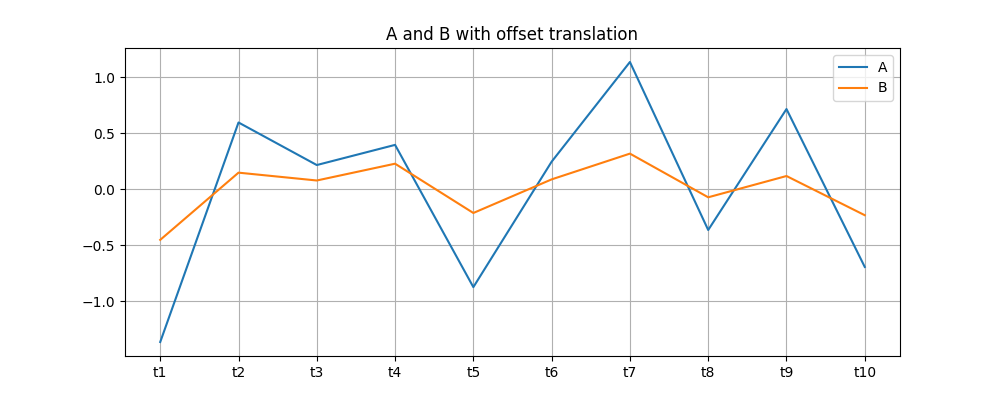
\includegraphics[width=\textwidth]{plots/offset_translation.png}

    Now, we take the results from offset translation and carry out amplitude scaling
    for both time series. Note that, in the python code in \autoref{appA} the function
    amp\_scaling() takes the raw data, not the translated data from the previous
    part to avoid any rounding errors during the calculation. We again have summarized
    the results in a table and plot. The distances based on the data after amplitude
    scaling are again calculated in the above demonstrated scheme:
    \begin{flalign*}
        \text{dist}_1 & = 1.7506937958804625 & \\
        \text{dist}_{\infty} & = 0.45459264054347487 & \\
    \end{flalign*}

    \hskip-2.0cm\begin{tabular}{c | c c c c c c c c c c}
        Series & \(t_1\) & \(t_2\) & \(t_3\) & \(t_4\) & \(t_5\) & \(t_6\) & \(t_7\) & \(t_8\) & \(t_9\) & \(t_{10}\) \\
        \hline
        A & \(-1.721128\) & \(0.750235\) & \(0.271093\) & \(0.498055\) & \(-1.103287\) & \(0.308920\) & \(1.431121\) & \(-0.460228\) & \(0.901543\) & \(-0.876325\) \\
        B & \(-1.901099\) & \(0.616913\) & \(0.323145\) & \(0.952648\) & \(-0.893894\) & \(0.365112\) & \(1.330350\) & \(-0.306358\) & \(0.491012\) & \(-0.977828\) \\
    \end{tabular}

    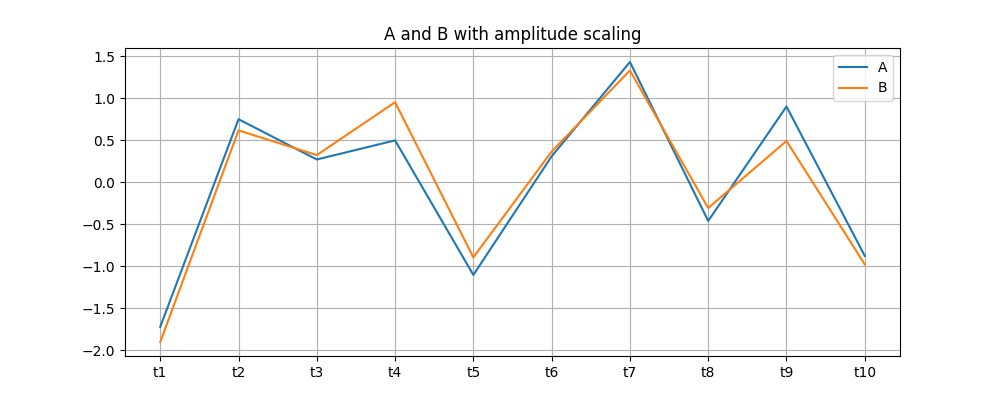
\includegraphics[width=\textwidth]{plots/amplitude_scaling.png}

    \pagebreak
    \section{Appendix A}
    \label{appA}
    \begin{lstlisting}
import pandas as pd

a = {'t1': -1.66, 't2': 0.30, 't3': -0.08, 't4': 0.10, 't5': -1.17, 't6': -0.05, 't7': 0.84, 't8': -0.66, 't9': 0.42, 't10': -0.99}
b = {'t1': 0.29, 't2': 0.89, 't3': 0.82, 't4': 0.97, 't5': 0.53, 't6': 0.83, 't7': 1.06, 't8': 0.67, 't9': 0.86, 't10': 0.51}

sera = pd.Series(data=a, index=['t1','t2','t3','t4','t5','t6','t7','t8','t9','t10'])
serb = pd.Series(data=b, index=['t1','t2','t3','t4','t5','t6','t7','t8','t9','t10'])

indexlist=['t1','t2','t3','t4','t5','t6','t7','t8','t9','t10']

# function to calculate manhatten distances
def man_dist(series1, series2):
    if series1.size == series2.size:
        result = []
        series1list = series1.to_list()
        series2list = series2.to_list()
        for i in range(0,series1.size-1):
            result = result + [abs(series1list[i] - series2list[i])]
        return sum(result)
    else:
        print("series not the same size, aborting")

# function to calculate max distance
def inf_dist(series1, series2):
    if series1.size == series2.size:
        result = []
        series1list = series1.to_list()
        series2list = series2.to_list()
        for i in range(0,series1.size -1):
            result = result + [abs(series1list[i] - series2list[i])]
        return max(result)
    else:
        print('series not the same size, aborting')

# task 1:
print('Results for task 1, calculating the distances for raw data:')

print('Manhatten Distance:')
print(man_dist(sera, serb))

print('Inf Distance:')
print(inf_dist(sera, serb))

# offset translation

def offset_translation(series, mean):
    result = []
    serieslist = series.to_list()
    for i in range(0,series.size):
        result = result + [(serieslist[i] - mean)]
    return pd.Series(result, index = indexlist)

sera_offset = offset_translation(sera, sera.mean())
serb_offset = offset_translation(serb, serb.mean())

print('Series A with offset translation:')
print(sera_offset)
print('Series B with offset translation:')
print(serb_offset)

sera_offset.name = 'A'
serb_offset.name = 'B'

amp_df = pd.merge(sera_offset,serb_offset,left_index=True,right_index=True)
plot = amp_df.plot(grid=True,figsize=(10,4),title='A and B with offset translation')
plot.set_xticks(range(len(amp_df)))
plot.set_xticklabels(["%s" % item for item in indexlist])
fig = plot.get_figure()
fig.savefig('plots/offset_translation.png')

print('Recalculating distances:')
print('Manhatten Distance:')
print(man_dist(sera_offset, serb_offset))
print('Inf Distance:')
print(inf_dist(sera_offset,serb_offset))

# amplitude scaling:
def amp_scaling(series):
    mean = series.mean()    # mean
    s = series.std()        # standard deviation
    result = []
    serieslist = series.to_list()
    for i in range(0,series.size):
        result = result + [(serieslist[i] - mean)/s]
    return pd.Series(result, index=indexlist)

sera_amp = amp_scaling(sera)
serb_amp = amp_scaling(serb)

print('Series A with amplitude scaling:')
print(sera_amp)
print('Series B with amplitude scaling:')
print(serb_amp)
print('Recalculate distances:')
print('Manhatten Distance:')
print(man_dist(sera_amp,serb_amp))
print('Inf Distance:')
print(inf_dist(sera_amp,serb_amp))

sera_amp.name = 'A'
serb_amp.name = 'B'

amp_df = pd.merge(sera_amp,serb_amp,left_index=True,right_index=True)
plot = amp_df.plot(grid=True,figsize=(10,4),title='A and B with amplitude scaling')
plot.set_xticks(range(len(amp_df)))
plot.set_xticklabels(["%s" % item for item in indexlist])
fig = plot.get_figure()
fig.savefig('plots/amplitude_scaling.png')
    \end{lstlisting}
    
\end{document}
